% ================= 附录开始 =================

\section{附录：实验原始记录日志}

\begin{figure}[H]
    \centering
    % 请确保你的图片文件在同一文件夹下，或者修改路径
    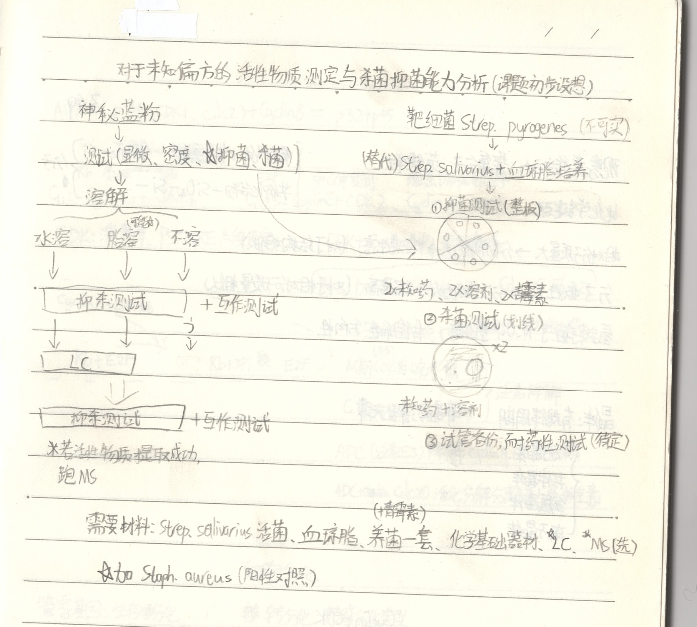
\includegraphics[width=0.8\textwidth]{figures/first_thoughts.png} 
    % \fbox{\begin{minipage}{0.8\textwidth}\centering 此处插入显微镜照片占位符 \end{minipage}}
    \caption{课题初步设想}
    \label{fig:first_thoughts}
\end{figure}

% 这里使用 longtable 制作跨页表格，防止日志太长被切断
\begin{longtable}{|c|c|p{3.5cm}|p{4.5cm}|p{3cm}|}
    \hline
    \textbf{日期} & \textbf{时间} & \textbf{操作/条件} & \textbf{现象/数据} & \textbf{备注} \\
    \hline
    \endfirsthead % 表格第一页的表头
    
    \hline
    \textbf{日期} & \textbf{时间} & \textbf{操作/条件} & \textbf{现象/数据} & \textbf{备注} \\
    \hline
    \endhead
    
    \hline
    \multicolumn{5}{|r|}{\textit{续下页...}} \\
    \endfoot
    
    \hline
    \endlastfoot % 表格最后一页的表尾

    % --- 日志内容开始 (直接复制修改这里) ---
    2023-10-01 & 09:00 & 配制 LB 培养基，灭菌 \SI{121}{\degreeCelsius} & 培养基澄清，无沉淀 & 批次 \#01 \\
    \hline
    2023-10-01 & 14:00 & 接种大肠杆菌，摇床培养 & 菌液略显浑浊 & 转速 \SI{200}{rpm} \\
    \hline
    2023-10-02 & 08:30 & 观察菌液浓度 (OD600) & OD 值 = 0.85 & 进入对数生长期 \\
    \hline
    2023-10-02 & 09:00 & 加入抑制剂 A (浓度 \SI{10}{mg/mL}) & 无明显变化 & 开始计时 \\
    \hline
    2023-10-02 & 12:00 & 取样涂布平板 & 菌落数量减少 & 见照片 Fig-A1 \\
    \hline

\end{longtable}

\section{附录：主要试剂配方}
\begin{itemize}
    \item \textbf{LB 培养基}: 胰蛋白胨 \SI{10}{g/L}, 酵母提取物 \SI{5}{g/L}, NaCl \SI{10}{g/L}.
    \item \textbf{缓冲液}: PBS (pH 7.4).
\end{itemize}

% ================= 附录结束 =================